% ============================================================
%  Experiment 3 --- Introduction to Altera Quartus II Software,
%  and Interfacing FPGA to DIP Switch and Seven Segment
%  (merged from the former Experiment 3 and Experiment 4)
% ============================================================
\experimentheader{3}{Experiment 3}{Introduction to Altera Quartus II Software, and Interfacing FPGA to DIP Switch and Seven Segment}{FPGA Lab}

\begin{objectives}
  \begin{enumerate}
    \item To use schematic entry as a design method in Altera Quartus II.
    \item To use Verilog as a design entry method in Altera Quartus II.
    \item To combine schematic and Verilog as a single design entry in Altera Quartus II.
    \item To simulate the circuit using Altera Quartus II.
    \item To download the design onto an Altera DE2 board.
    \item To interface a DIP switch and a seven-segment display to the FPGA.
  \end{enumerate}
\end{objectives}

\begin{equipment}
  \begin{enumerate}
    \item Altera Quartus II software
          \begin{itemize}
            \item version 9/10/12 for Cyclone II
            \item version 9/10/12/latest for Cyclone IV
          \end{itemize}
    \item Altera DE2 board
    \item Function generator
  \end{enumerate}
\end{equipment}

\begin{introduction}
  Seven-segment displays are widely used to show numbers. The DE2 board provides eight seven-segment displays, 18 DIP switches, four push-button switches, and 16 LEDs. These components are hardwired on the board and are each assigned to specific FPGA pins --- refer to the DE2 user manual for the full pin map.
\end{introduction}

\begin{procedure}

  \textbf{Activity 1 --- Schematic entry}\vspace{2pt}

  \textit{Objective: use schematic entry to design a 4-to-1 multiplexer in Quartus II.}

  \begin{enumerate}
    \item Open Quartus II and start the New Project Wizard.
          \begin{itemize}
            \item Working directory: \texttt{fpga}; project name: \texttt{activity1}; top-level entity: \texttt{mux\_sch}.
            \item Device family: Cyclone II (\texttt{EP2C35F672C6N}) or Cyclone IV (\texttt{EP4CE115F29C7N}).
            \item Accept the default EDA tool settings (synthesis, simulation, timing analysis) and finish.
          \end{itemize}
    \item Create a new Block Diagram/Schematic file.
    \item Place three 3-input AND gates and one 4-input OR gate from the primitives library, and wire them as shown in Figure~\ref{fig:exp3-mux-schematic} using rubberbanding to connect components.
    \item Add and name the input pins (\texttt{i0}--\texttt{i3}, \texttt{s0}, \texttt{s1}) and the output pin (\texttt{out}).
    \item Save as \texttt{mux\_sch.bdf} and start compilation.
    \item Create a Vector Waveform File to simulate the design: insert input nodes \texttt{i0}--\texttt{i3}, \texttt{s0}, \texttt{s1}, and output node \texttt{out}.
    \item Assign logic values to the inputs, save as \texttt{mux\_sch.vwf}, then run Compilation and Simulation.
    \item Record the outputs, then repeat for each input combination in Table~\ref{tab:exp3-truth}, saving the waveform file each time.
    \item Print and submit the schematic diagram and simulation result.
  \end{enumerate}

  \begin{boxedfigure}
    \centering
    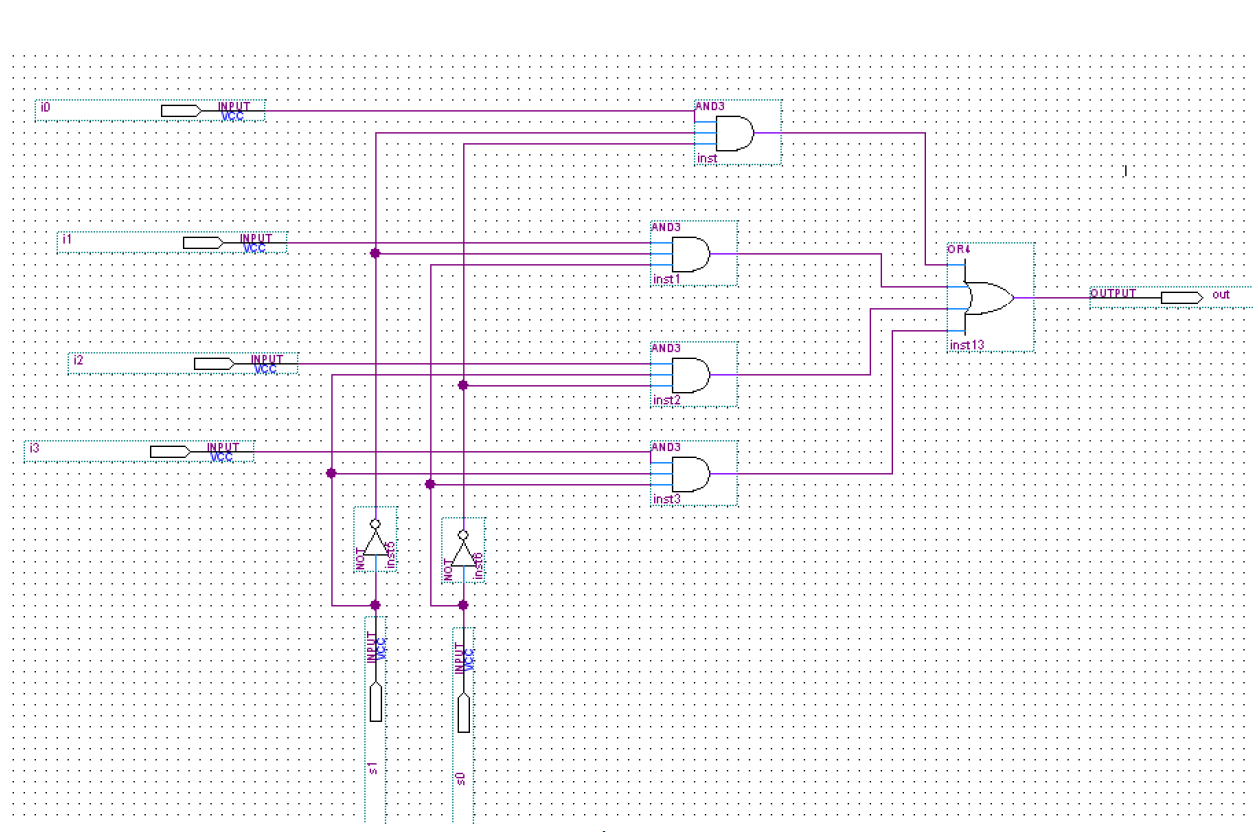
\includegraphics[width=0.85\linewidth]{figures/Exp3_Figure_1.png}
    \captionof{figure}{Mux Schematic.}
    \label{fig:exp3-mux-schematic}
  \end{boxedfigure}

  \needspace{4cm}
  \begin{boxedtable}
    \captionof{table}{Input combinations to simulate.}
    \label{tab:exp3-truth}
    {\renewcommand{\arraystretch}{1.5}
      \centering
      \begin{tabular}{cccccc}
        \toprule
        S0 & S1 & I0 & I1 & I2 & I3 \\
        \midrule
        0  & 0  & 1  & 1  & 0  & 0  \\
        0  & 1  & 0  & 1  & 1  & 0  \\
        1  & 0  & 1  & 1  & 0  & 1  \\
        1  & 1  & 1  & 1  & 0  & 0  \\
        \bottomrule
      \end{tabular}
    }
  \end{boxedtable}
  \vspace*{1.5em}

  \textbf{Activity 2 --- Verilog entry}\vspace{2pt}

  \textit{Objective: use Verilog code as a design entry method in Quartus II.}

  \begin{enumerate}
    \item Start a new project (\texttt{Activity2}, top level \texttt{mux\_ver}) with the same device and EDA tool settings as Activity 1.
    \item Create a new Verilog file and enter the code in Listing~\ref{lst:exp3-mux-ver}.
    \item Save as \texttt{mux\_ver}, then compile the design.\newpage
    \item Create a Vector Waveform File; insert input nodes \texttt{i0}--\texttt{i3}, \texttt{s0}, \texttt{s1}, and output node \texttt{out}.
    \item Assign logic values matching Table~\ref{tab:exp3-truth}, save as \texttt{mux\_ver.vwf}, then start simulation.
    \item Inspect the result in the Simulation Report --- Simulation Waveform.
    \item Change the input values (saving before each run) and re-simulate.
    \item View the synthesized schematic via \textbf{Tools} $\to$ \textbf{Netlist Viewer} $\to$ \textbf{RTL Viewer}, shown in Figure~\ref{fig:exp3-rtl}.
    \item Print and submit the Verilog code and simulation result.
  \end{enumerate}

  \begin{codepanel}{mux\_ver.v}{verilogstyle}
    \begin{lstlisting}
module mux_ver(out, i0, i1, i2, i3, s1, s0);
  output out;
  input i0, i1, i2, i3;
  input s1, s0;
  reg out;

  always @(s1 or s0 or i0 or i1 or i2 or i3)
  begin
    case ({s1, s0})
      2'b00: out = i0;
      2'b01: out = i1;
      2'b10: out = i2;
      2'b11: out = i3;
      default: out = 1'bx;
    endcase
  end
endmodule
\end{lstlisting}
  \end{codepanel}
  \vspace{-4pt}
  \listingcaption{lst:exp3-mux-ver}{\texttt{mux\_ver.v} --- Verilog 4-to-1 multiplexer.}

  \begin{boxedfigure}
    \centering
    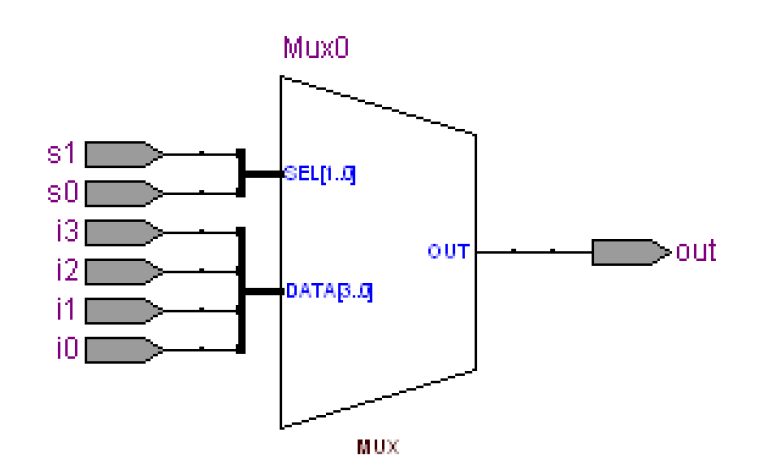
\includegraphics[width=0.75\linewidth]{figures/Exp3_Figure_2.png}
    \captionof{figure}{RTL Viewer output for \texttt{mux\_ver} (\texttt{Mux0}).}
    \label{fig:exp3-rtl}
  \end{boxedfigure}
  \newpage

  \textbf{Activity 3 --- Combining schematic and Verilog entry}\vspace{2pt}

  \textit{Objective: combine a Verilog module with schematic entry in a single design.}

  \begin{enumerate}
    \item Start a new project (\texttt{activity3}, top level \texttt{mux\_schver}) with the same device and EDA tool settings.
    \item Create a new Verilog HDL file with the code in Listing~\ref{lst:exp3-mux-vrl}; save as \texttt{mux\_vrl}.
    \item Generate a reusable symbol from the file via \textbf{File} $\to$ \textbf{Create/Update} $\to$ \textbf{Create Symbol Files for Current File}. The resulting block is shown in Figure~\ref{fig:exp3-mux-vrl-symbol}.
    \item Create a new Block Diagram/Schematic file, place the \texttt{mux\_vrl} symbol from the project library, and connect its inputs and output to input/output pads as shown in Figure~\ref{fig:exp3-mux-schver}.
    \item Save as \texttt{mux\_schver.bdf} and start compilation.
    \item Create a Vector Waveform File, insert the same nodes as before, assign logic values, save as \texttt{mux\_schver.vwf}, and run Compilation and Simulation.
    \item Record the outputs for the combinations in Table~\ref{tab:exp3-truth}, saving the waveform file each time.
    \item Print and submit the schematic diagram, Verilog code, and simulation result.
  \end{enumerate}

  \begin{codepanel}{mux\_vrl.v}{verilogstyle}
    \begin{lstlisting}
module mux_vrl(out, i0, i1, i2, i3, s1, s0);
  output out;
  input i0, i1, i2, i3;
  input s1, s0;
  reg out;

  always @(s1 or s0 or i0 or i1 or i2 or i3)
  begin
    case ({s1, s0})
      2'b00: out = i0;
      2'b01: out = i1;
      2'b10: out = i2;
      2'b11: out = i3;
      default: out = 1'bx;
    endcase
  end
endmodule
\end{lstlisting}
  \end{codepanel}
  \vspace{-4pt}
  \listingcaption{lst:exp3-mux-vrl}{\texttt{mux\_vrl.v} --- Verilog module to be reused as a schematic symbol.}

  \begin{boxedfigure}
    \centering
    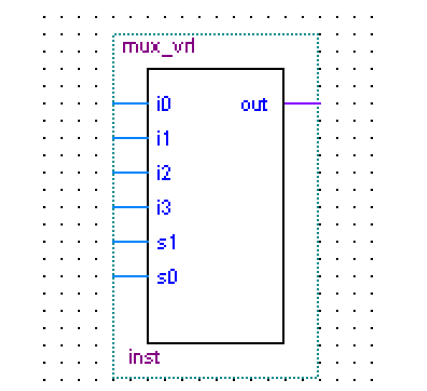
\includegraphics[width=0.85\linewidth]{figures/Exp3_Figure_3.png}
    \captionof{figure}{Auto-generated \texttt{mux\_vrl} symbol block.}
    \label{fig:exp3-mux-vrl-symbol}
  \end{boxedfigure}
  \vspace*{1em}

  \begin{boxedfigure}
    \centering
    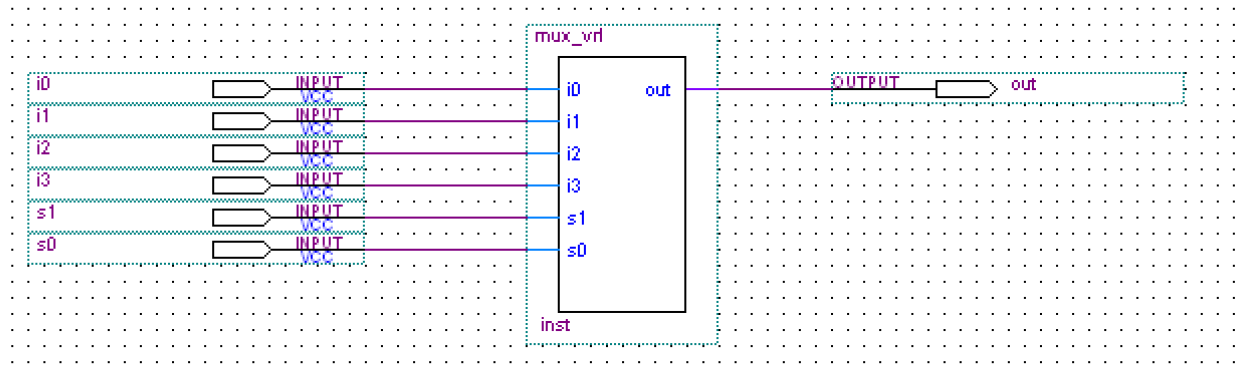
\includegraphics[width=\linewidth]{figures/Exp3_Figure_4.png}
    \captionof{figure}{Combined schematic \texttt{mux\_schver}.}
    \label{fig:exp3-mux-schver}
  \end{boxedfigure}
  \vspace*{1em}

  \textbf{Activity 4 --- Timing analysis}\vspace{2pt}

  \textit{Objective: analyse the maximum operating speed of a design.}

  \begin{enumerate}
    \item Start a new project (\texttt{Activity4}, top level \texttt{counter}) with the same device and EDA tool settings.
    \item Create a new Verilog file with the code in Listing~\ref{lst:exp3-counter}; save as \texttt{counter} and compile.
    \item Create a Vector Waveform File; insert \texttt{clock} and \texttt{clear} as inputs and \texttt{Q} as output.
    \item Force \texttt{clear} low, assign a clock signal to \texttt{clock}, save as \texttt{counter.vwf}, then start simulation.
    \item Inspect the result in the Simulation Report --- Simulation Waveform.
    \item Run \textbf{Processing} $\to$ \textbf{Start} $\to$ \textbf{Start Classic Timing Analyzer}.
    \item Read the maximum clock frequency from the Timing Analyzer Summary (Figure~\ref{fig:exp3-timing}).
    \item Print and submit the Verilog code and simulation result.
  \end{enumerate}

  \begin{codepanel}{counter.v}{verilogstyle}
    \begin{lstlisting}
module counter(Q, clock, clear);
  output [3:0] Q;
  input clock, clear;
  reg [3:0] Q;

  always @(posedge clear or negedge clock)
  begin
    if (clear)
      Q = 4'd0;
    else
      Q = (Q + 1) % 16;
  end
endmodule
\end{lstlisting}
  \end{codepanel}
  \vspace{-4pt}
  \listingcaption{lst:exp3-counter}{\texttt{counter.v} --- 4-bit up counter with asynchronous clear.}
  \vspace*{1em}

  \begin{boxedfigure}
    \centering
    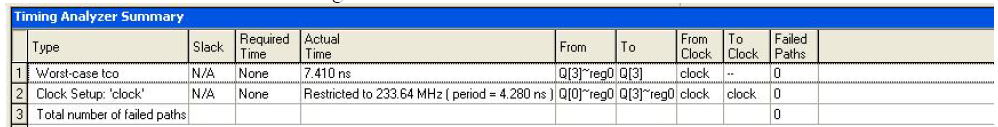
\includegraphics[width=\linewidth]{figures/Exp3_Figure_6.png}
    \captionof{figure}{Timing analyzer summary for the \texttt{counter} design.}
    \label{fig:exp3-timing}
  \end{boxedfigure}
  \vspace*{1em}

  \textbf{Activity 5 --- Downloading to the DE2 board}\vspace{2pt}

  \textit{Objective: download a Verilog design onto the Altera DE2 board and drive the seven-segment display.}

  \begin{enumerate}
    \item Start a new project (\texttt{activity5}, top level \texttt{counta}) with the same device and EDA tool settings.
    \item Create a new Verilog HDL file with the code in Listing~\ref{lst:exp3-counta}; save as \texttt{counta}.
    \item Compile and simulate the design.
    \item Assign each output pin to a physical device pin using \textbf{Assignment} $\to$ \textbf{Pin Planner}, per Table~\ref{tab:exp3-pins} (refer to the DE2 user manual for pin locations).
    \item Save, then recompile the project.
    \item Download the configuration to the DE2 board via \textbf{Tools} $\to$ \textbf{Programmer} $\to$ \textbf{Hardware Setup} $\to$ USB-Blaster $\to$ \textbf{Start}.
    \item Record the pattern displayed on the seven-segment display.
    \item Change the assignment to \verb|assign q[6:0] = 7'b1111000;|, save, recompile, and download again. Record the new displayed pattern.
  \end{enumerate}

  \begin{codepanel}{counta.v}{verilogstyle}
    \begin{lstlisting}
module counta(q);
  output [6:0] q;
  assign q[6:0] = 7'b0010000;
endmodule
\end{lstlisting}
  \end{codepanel}
  \vspace{-4pt}
  \listingcaption{lst:exp3-counta}{\texttt{counta.v} --- static seven-segment pattern.}

  \needspace{4cm}
  \begin{boxedtable}
    \captionof{table}{Seven-segment output pin assignment (DE2 board).}
    \label{tab:exp3-pins}
    {\renewcommand{\arraystretch}{1.5}
      \centering
      \begin{tabular}{cccc}
        \toprule
        \# & Node name & Direction & Pin \\
        \midrule
        1  & Q[6]      & Output    &     \\
        2  & Q[5]      & Output    &     \\
        3  & Q[4]      & Output    &     \\
        4  & Q[3]      & Output    &     \\
        5  & Q[2]      & Output    &     \\
        6  & Q[1]      & Output    &     \\
        7  & Q[0]      & Output    &     \\
        \bottomrule
      \end{tabular}
    }
  \end{boxedtable}
  \vspace*{1.5em}

  \textbf{Activity 6 --- 16-bit binary counter with frequency divider}\vspace{2pt}

  \textit{Objective: design a 16-bit binary counter driven through a frequency divider.}

  \begin{enumerate}
    \item Open Quartus II and write the frequency-divider module in Listing~\ref{lst:exp3-seven} (\texttt{seven}), which lowers the incoming clock frequency (Device family: Cyclone II (\texttt{EP2C35F672C6N}) or Cyclone IV (\texttt{EP4CE115F29C7N})).
    \item Create a reusable symbol for \texttt{seven}.
    \item Write the 4-bit counter module in Listing~\ref{lst:exp3-led} (\texttt{led}).
    \item Create a reusable symbol for \texttt{led}.
    \item Draw the schematic in Figure~\ref{fig:exp3-schematic4}, connecting the \texttt{seven} block's most significant output bit \texttt{q[16]} to the clock input of the \texttt{led} block.
    \item Assign pin numbers as shown in Table~\ref{tab:exp3-pins4} (refer to the DE2 user manual).
    \item Use a function generator to supply the clock signal, using 1\,MHz as the clock input.
    \item Determine the effective input frequency reaching the \texttt{led} module.
    \item Discuss your result based on the observed LED output display.
  \end{enumerate}

  \begin{codepanel}{seven.v --- frequency divider}{verilogstyle}
    \begin{lstlisting}
module seven(q, clk);
  output [15:0] q;
  input clk;
  reg [15:0] q;

  always @(posedge clk)
  begin
    q = (q + 1) % 65536;
  end
endmodule
\end{lstlisting}
  \end{codepanel}
  \vspace{-4pt}
  \listingcaption{lst:exp3-seven}{\texttt{seven.v} --- 16-bit frequency divider.}

  \begin{codepanel}{led.v --- 4-bit counter}{verilogstyle}
    \begin{lstlisting}
module led(x, clk);
  input clk;
  output [3:0] x;
  reg [3:0] x;

  always @(posedge clk)
  begin
    x = (x + 1) % 16;
  end
endmodule
\end{lstlisting}
  \end{codepanel}
  \vspace{-4pt}
  \listingcaption{lst:exp3-led}{\texttt{led.v} --- 4-bit binary counter.}

  \begin{boxedfigure}
    \centering
    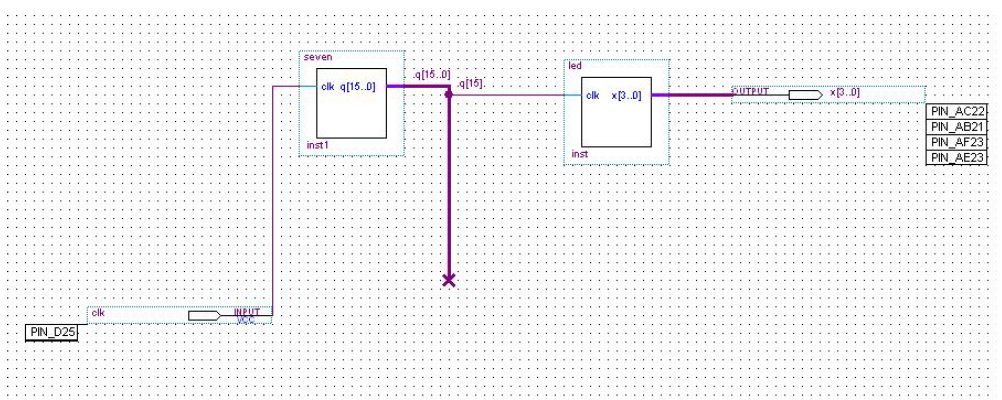
\includegraphics[width=0.85\linewidth]{figures/Exp4_Figure_1.png}
    \captionof{figure}{Schematic diagram for the 16-bit binary counter with frequency divider.}
    \label{fig:exp3-schematic4}
  \end{boxedfigure}

  \needspace{4cm}
  \begin{boxedtable}
    \captionof{table}{Pin assignment for the 4-bit binary counter.}
    \label{tab:exp3-pins4}
    {\renewcommand{\arraystretch}{1.5}
      \centering
      \begin{tabular}{cccc}
        \toprule
        \# & Node name & Direction & Pin location \\
        \midrule
        1  & clk       & Input     &              \\
        2  & X[3]      & Output    &              \\
        3  & X[2]      & Output    &              \\
        4  & X[1]      & Output    &              \\
        5  & X[0]      & Output    &              \\
        \bottomrule
      \end{tabular}
    }
  \end{boxedtable}
  \vspace*{1.5em}

  \textbf{Activity 7 --- 0--99 counter on seven-segment display}\vspace{2pt}

  \textit{Objectives: (1) design a counter that counts 0 to 99; (2) display the result on the seven-segment displays.}

  \begin{enumerate}
    \item Using a DIP switch as the trigger input, write Verilog code for a counter that counts from 0 to 99 once the switch is triggered.
    \item Decode and display the result (tens and units digits) on two seven-segment displays.
    \item Print and submit the Verilog code and simulation result.
  \end{enumerate}
  \vspace*{1em}

  \textbf{Activity 8 --- Running light}\vspace{2pt}

  \textit{Objective: design a running-light display on the Altera DE2 board.}

  \begin{enumerate}
    \item Using a DIP switch as the input, write Verilog code to implement a running-light (chasing LED) pattern.
    \item Use three DIP switches to select between three different running-light patterns.
    \item Print and submit the Verilog code and simulation result.
  \end{enumerate}

\end{procedure}
